\documentclass[a4pape, 11pt, english]{article}
\usepackage[margin=1in,footskip=0.25in]{geometry}
\usepackage{natbib}

%\usepackage{cite}
\usepackage{amsmath,amssymb,amsfonts}
\usepackage{algorithmic}
\usepackage{graphicx}
\usepackage{textcomp}
\usepackage{xcolor}

\usepackage[hyphens]{url} % To wrap urls on multiple lines: https://tex.stackexchange.com/questions/115690/urls-in-bibliography-latex-not-breaking-line-as-expected

\def\BibTeX{{\rm B\kern-.05em{\sc i\kern-.025em b}\kern-.08em
    T\kern-.1667em\lower.7ex\hbox{E}\kern-.125emX}}

\begin{document}
\title{Deep Reinforcement Learning Project}
\author{Thomas Fishwick}
\date{} % hide the date
\maketitle

\begin{abstract}
TODO: Abstract

Our code is available at this link \url{https://github.com/SL477/DRL-coursework}.
\end{abstract}

\section{Main problem: Starship Saboteur}
% describe the q-learning algorithm and my implementation of it
% describe some key parameters
\subsection{Define an environment and the problem to be solved}
%Here our agent will be teleported into a random free location on a spaceship (i.e. not blocked by any obstacles). Our agent will need to disable the spaceship's reactor by standing upon a certain location. Avoid the traps (which deal damage when stepped on) and navigate through the ship. Then go to the random beam-out location (which will also be an empty square) and escape before the max allowed turns, after that the ship will open the airlocks to immediately kill the agent.

%The agent will be able to 'see' the area around it not blocked by walls/other obstacles. Doors will count as obstacles to vision, but not to the agent. Its next objective's direction will be fed to it, along with its current health.

Our agent will start in a random empty location in the map shown in Figure \ref{fig:basic_map}. It has two positive reward points, the darker green point is the one with the highest reward and the lighter green point will terminate the training episode. The yellow points are negative reward points, they also deduct health points and if the agent's health drops to zero or less this will also terminate the episode. The agent can transition to any adjacent cell as long as it is not a wall. Currently the doors are only decorative items.

\textbf{The story version:}
Fired from a Solar Federation Space Force Infiltrator, our intrepid Space Marine Commando robot exits its boarding pod in a random place in the Custodian warship. Its mission is to cripple the ship's reactor before its crew are revived from stasis by planting a timed explosive on it. Its survival is optional, after it has completed its mission the robot can escape back to where a shuttle has cut a hole into the ship to retrieve it. But if the robot is destroyed, well we can always build more robots.
% harpoon line has been fired into the ship to retrieve it.

We will be using Q-learning to 'solve' this environment. Q-learning attempts to work out the cost/benefit of going from one state to the various other states around it based on their current and future rewards. Figure \ref{fig:basic_map_graph} shows which nodes are accessible to each other.

\begin{figure}[h!]
	\begin{center}
		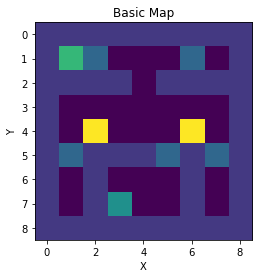
\includegraphics{img/basic_map.png}
		\caption{Green: reward points, yellow: obstacles, blue: doors, dark purple: empty space, light purple: walls}
		\label{fig:basic_map}
	\end{center}
\end{figure}

\begin{figure}[h!]
	\begin{center}
		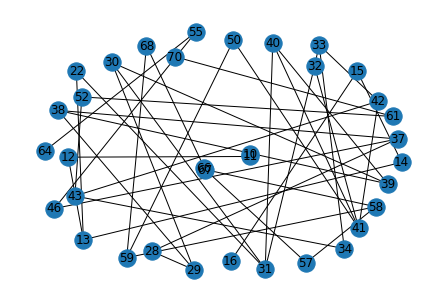
\includegraphics[scale=0.5]{img/basic_map_graph.png}
		\caption{Nodes with access to one another}
		\label{fig:basic_map_graph}
	\end{center}
\end{figure}


\subsection{Define a state transition function and the reward function}
To make our list of states we flatten the 2D map into an array. To flip from the array to the map we can get the row by integer dividing the index by the height of the map and the column by taking the modulus of the index by the width.

For the reward function we create a matrix with one state per row and one action per column. Using a lookup back to the map we get the code of the cell and lookup its reward (table \ref{tab:table1}). As the agent is only allowed to claim the primary objective once per episode the reward is set to zero once it has been claimed by the agent.

\begin{table}[h!]%[htbp]
	\begin{center}
		\caption{Rewards}
		\label{tab:table1}
		\begin{tabular}{|c|c|}
			\hline
			\textbf{Code} & \textbf{Reward} \\
			\hline
			Empty space & 0 \\
			\hline
			Wall & 0 \\
			\hline
			Door & 0 \\
			\hline
			The primary goal (the reactor control panel) & 50 \\
			\hline
			The secondary goal (the escape route) & 30 \\
			\hline
			A trap & -10 \\
			\hline
		\end{tabular}
	\end{center}
\end{table}



\subsection{Set up the Q-learning parameters (gamma, alpha) and policy}
For the Q-learning algorithm we have implemented it as a function (run\_q\_learning\_basic), with the parameters alpha, gamma, epsilon and num episodes.

Alpha, the learning rate, we have set as 1.

Gamma, the discount factor for future rewards, we set as 0.8.

Epsilon, the chance of choosing the policy 'exploit' over 'explore', we set as 0.9.

Num\_episodes, the number of learning episodes, we set as 1000.

\subsection{Run the Q-learning algorithm and represent its performance}
The Q-learning algorithm is:

$Q[s, a] = Q[s, a] + \alpha * R[s, a] + \gamma * (max(Q[s]) - Q[s, a])$

With the exploit/explore part given by:

if RandomNumber $> \epsilon$ then explore, otherwise exploit.

The algorithm takes 22.5 seconds to run on my PC. In Figure \ref{fig:firstparamsRewardVQVar} we can see the mean rewards versus their corresponding Q variances. The mean total health stayed at roughly 100, with at least one iteration within each iteration doing something to reduce its health. Most of the iteration's mean rewards were around 50, indicating that they were only going for one of the reward points (fortunately the higher reward point).

\begin{figure}[h!]
	\begin{center}
		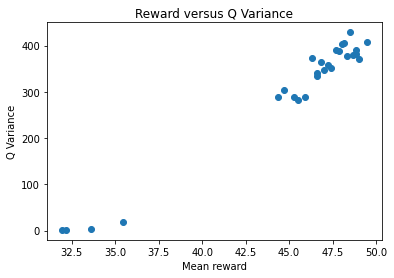
\includegraphics[scale=0.8]{img/firstparamsRewardVQVarWithEarlyStopping.png}
		\caption{Reward Versus Variance, for Alpha = 1, Gamma = 0.8, Epsilon = 0.9, for 27 rounds of 1000 iterations of training}
		\label{fig:firstparamsRewardVQVar}
	\end{center}
\end{figure}

It also looks like those which converged fastest were also the ones to get the lowest reward (around 30), they likely found that one first and did not explore enough to find the other reward point.

\subsection{Repeat the experiment with different parameter values, and policies}
Running a full grid search of Alpha, Gamma and Epsilon parameters results in Figure \ref{fig:GridSearchColorGamma}, where we can see that as the epsilon (explore/exploit) parameter gets lower (promoting explore) our agent is more likely to wander into one or more of the traps. Considering that these traps give minus ten points and this is the average reward over the number of episodes until convergence (or 1000 episodes) this is quite the effect for some of the more extreme negative rewards (the agent can only step on the traps ten times a run before it is terminated).

\begin{figure}[h!]
	\begin{center}
		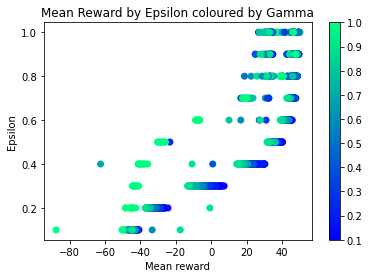
\includegraphics[scale=0.8]{img/GridSearchRewardEpsilonGamma.png}
		\caption{Grid Search of the parameters}
		\label{fig:GridSearchColorGamma}
	\end{center}
\end{figure}

Holding the other parameters stationary and running through the different Gamma (discount factor for future reward) sees a steady decline in how much reward it picks up, until at Gamma equals 1 (or in other words future rewards are now worthless) it repeatedly throws itself at the traps (Figure \ref{fig:GridSearchGamma}). We had it run through a thousand episode training session three times for each parameter, so it is not that likely to be a statistical anomoly.

\begin{figure}[h!]
	\begin{center}
		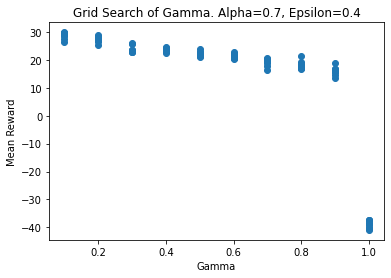
\includegraphics[scale=0.5]{img/GridSearchGamma.png}
		\caption{Grid Search of the gamma parameter}
		\label{fig:GridSearchGamma}
	\end{center}
\end{figure}

For Alpha (the learning rate) running a grid search with Gamma at 0.8 and Epsilon at 0.4, does not seem to have too much effect on the mean reward but it does have a more or less linear relationship with the Q variance (the Gamma variable has a similar effect up until gamma = 1) as shown in Figure \ref{fig:GridSearchAlpha}.

\begin{figure}[h!]
	\begin{center}
		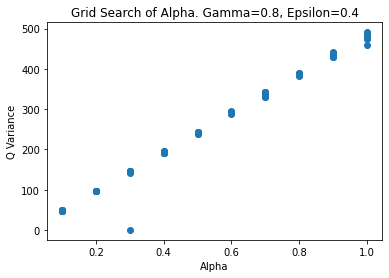
\includegraphics[scale=0.5]{img/GridSearchAlphaQ.png}
		\caption{Grid Search of the alpha parameter}
		\label{fig:GridSearchAlpha}
	\end{center}
\end{figure}

\subsection{Analyse the results quantitatively and qualitatively}
Here we compare the Q variance and mean rewards for the old parameters (Alpha: 1, Gamma: 0.8, Epsilon: 0.9) and the new parameters (Alpha: 0.8, Gamma: 0.8, Alpha: 0.4), in Figure \ref{fig:bothData}. The new parameters have much lower variance compared with the new parameters in that they are very tightly distributed and the old parameters are much more spread out. The problem with the new parameters is that they seem to be very good at learning the wrong lessons, as they have learnt to go for the lower reward by going through the traps. The original parameters have learnt to generally avoid the traps and some have gone for the higher reward point and some have gone for the lower reward point. The new values have high precision, but are somewhat biased away from what we want them to do (get the higher reward point and ideally the lower one too). The old values have low precision, but are generally unbiased towards their primary target (though some get just the secondary target, but not both).

%\begin{figure}[h!]
%	\begin{center}
%		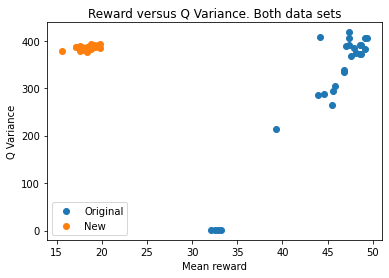
\includegraphics[scale=0.5]{img/bothDataRewardVQVar.png}
%		\caption{New Versus Old parameters}
%		\label{fig:bothDataRewardVQVar}
%	\end{center}
%\end{figure}

%\begin{figure}[h!]
%	\begin{center}
%		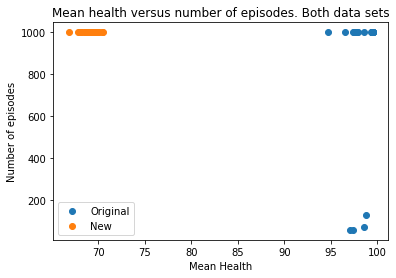
\includegraphics[scale=0.5]{img/bothDataHealthVNumEpisodes.png}
%		\caption{New Versus Old parameters}
%		\label{fig:bothDataHealthVNumEpisodes}
%	\end{center}
%\end{figure}

\begin{figure}[h!]
	\begin{center}
		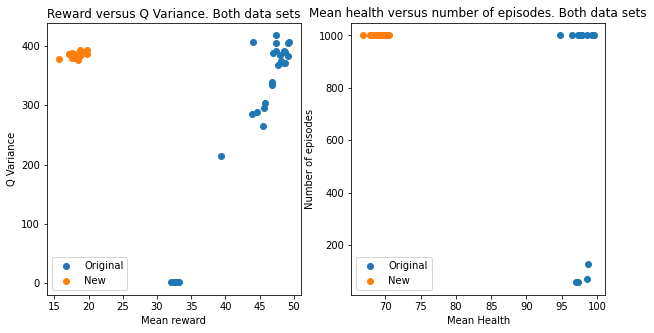
\includegraphics[scale=0.8]{img/bothData.png}
		\caption{New Versus Old parameters}
		\label{fig:bothData}
	\end{center}
\end{figure}

\section{Implement DQN with two improvements}
\begin{figure}[h!]
	\begin{center}
		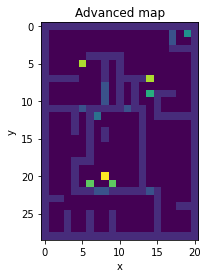
\includegraphics{img/advanced_map.png}
		\caption{Green: reward points, yellow: obstacles, blue: doors, dark purple: empty space, light purple: walls}
		\label{fig:advanced_map}
	\end{center}
\end{figure}

Here we have used a similar environment to the basic task, but now have enemies which move around and we now only have a limited field of view (Fig. \ref{fig:advanced_map}). To counter the limited field of view we have an objective compass to see where we are going. Our agent also has a gun to remove nearby enemies. Running the unimproved model through 44 variations of parameters leaves us with the best hidden units of 256 and 256, and the best gamma of 0.9.

\subsection{DQN with two improvements}
We will improve on the basic Q learning algorithm using two methods:

Our first one is Double Q-Learning. "The standard DQN uses the same values both to select and to evaluate an action. This makes it likely to select overestimated values, resulting in overoptomistic value estimates" \citep[p. 2]{van_hasselt_deep_2016}. As our environment is rather complicated we would not want the algorithm to over-estimate what it is doing, but to make sensible decisions about where to go and what to do. In the standard algorithm we have seen it improve, get worse and then improve again, so we would prefer to see continuous improvements in the algorithm's behaviour.

Our second improvement will be Prioritised Experience Replay, "an issue with traditional RL techniques is the potential rapid forgetting of possibly rare experiences that would be useful later on" \citep[p 1]{schaul_prioritized_2015}. Our environment is fairly large and only has two reward points, so it would be beneficial for the agent to remember to collect them (and in the correct order, as one point ends the episode so that it cannot collect the other one). The environment also has traps and enemies which it would be best to learn to avoid. A large portion of an episode would be moving from the start point to the reward points with not much else happening, it seems silly that the agent would remember those experiences with the same importance.

\subsection{Analyse the results quantitatively and qualitatively}

\begin{figure}[h!]
	\begin{center}
		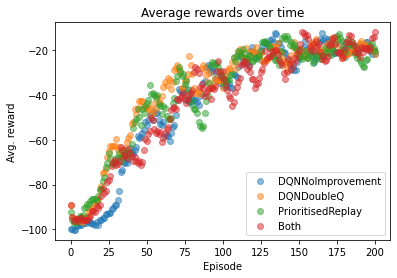
\includegraphics{img/DQNRewardsOverTime.png}
		\caption{DQN Rewards over time}
		\label{fig:DQNRewardsOverTime}
	\end{center}
\end{figure}

\begin{figure}[h!]
	\begin{center}
		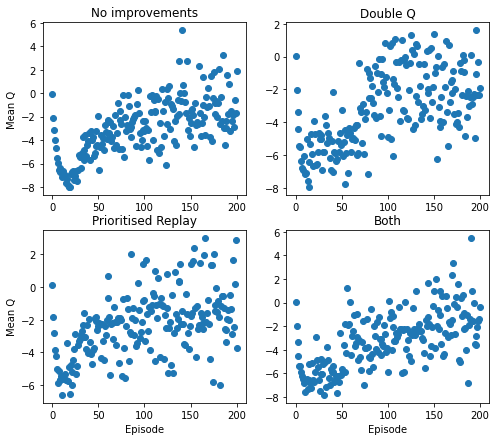
\includegraphics{img/DQNMeanQs.png}
		\caption{DQN Mean Q Values}
		\label{fig:DQNMeanQs}
	\end{center}
\end{figure}

From the rewards over time data we can see that all four models stayed in the range -100 to -12 for their mean rewards (meaning that we may have not been generous enough in our rewards for the AI). We took off one point per step, ten points off for hitting a trap or being hit by an enemy, we gave fifty points for the primary object and thirty points for the secondary objective. In Fig. \ref{fig:DQNRewardsOverTime} we can see that the Deep Q Network with no improvement took the longest to get started, then had a few ups and downs as it got to its minimum point (aside from a few sessions where it stayed around -100 the entire time this was generally how this one worked itself out). Double Q, Prioritised replay and both together all had something of a false start where they started around -90, then got worse and then got better. In the video of the one with no improvement we can see it going for the primary objective and then getting trapped against the wall, it may not have been properly able to distinguish between walls and doors, which are in the game terms one number from each other (in one of the other videos it went straight for the escape point). In Fig. \ref{fig:DQNMeanQs} we can see that the mean Q values for the agent, after a false start, generally tended upwards but in a very loose pattern.
Double Q had the most rapid improvement, although it also ossilated slighly up and down, but less violently than any of the others. Perhaps the prioritised replay emboldened it into making silly decisions when they were both together, as along it seemed to have less ossilations. This maybe because as double Q is designed not to overestimate actions it was able to more quickly learn what it needed to do. In the video of the Double Q agent we can see that it killed the enemy in the engine room before collecting the primary objective, whereas the more basic agent ignored/avoided it (whether it had not worked out what the gun did or decided not to waste a point in killing it is hard to tell). From the mean Q values in Fig. \ref{fig:DQNMeanQs} we can see that there was not too much of a pattern, except that they fell for the first few rounds.
Prioritised replay seemed to fall into two patterns of graph, the ones such as the one in Fig. \ref{fig:DQNRewardsOverTime} where it learned to get the reward fairly quickly and others where it did not appear to learn anything for quite a while and then cottened onto the fact that it needed to pick up the rewards. Out of all of the graphs it had the most violent downturn away from the reward, before getting back on track and fairly tightly following its minimum point. In the video we can see the agent fairly confidently grabbing the primary objective, but then it goes all wrong with the agent repeatedly slamming itself against the wall near the enemy. It maybe that it had not worked out about its gun and just knew to get out of the enemy's way rather than lose a point. In Fig. \ref{fig:DQNMeanQs} we can see that prioritised replay had the most tightly clustered Mean Q values, but apart from them trending down for the first few episodes they appear fairly randomly distributed.
For both improvements together we can see that its rewards improved the slowest, it appeared to ossilate the most from the curve but more gently than Prioritised Replay's or no improvement's. Perhaps showing the caution of prioritised Replay from some of its training session, but when it does learn something new not wildly swinging around as the Double Q side tempers it. In the video we can see that it started in the corridor above the engine room and made a beeline straight for the extraction point (leaving on a reward of 10, while all the other videos finished on -51). We can see that it had figured out that the exit point was directly at the top. However in the video Both2 we can see the agent in the engine room, killing the enemy, completing the objective and then jamming itself in the corner, so while it may have figured out the compass figures it does not seem to have figured out the difference between walls and doors (a door was very close to it, but led to a deadend, it may not have picked up how to navigate the ship, as the main entrance to the engine room is the only entrance and outside of the engine room it is relatively easy to work your way around to the exit point). In Fig. \ref{fig:DQNMeanQs} we can see that having both improvements meant that the mean Q values more or less followed the same loose pattern as the one with no improvements (possibly for this graph the two improvements were able to cancel each other out).

\section{Apply the RL algorithm of your choice (from rllib) to one of the Atari Learning Environment. Briefly present the algorithm and justify your choice}
In this section we chose to use the Evolutions Strategies algorithm and apply it onto the Space Invaders environment. Evolution Strategies is rather different to the Deep Q Network, in Deep Q Networks we have a neural network and after each episode of playing the game we will use gradient descent to adjust the weights of the neural network to try to improve the same network in the next episode of playing the game (roughtly inspired by the idea of how a brain learns). In Evolution Strategies, "a population of parameter vectors is peturbed and their objective function is evaluated. The highest scoring parameter vectors are then recombined to form the population for the next generation" \citep{salimans_evolution_2017}. Or in orther words it builds a series of random neural networks based on the prior generation (or a random seed for the first run) and the best one is then used to spawn another generation until the overall optimisation algorithm descides that it cannot get any better (taking its inspiration from evolution by natural selection).
The upshot of the algorithm is that it is embarressingly parallel, in  \citep{salimans_evolution_2017}[p. 7-8] the authors talk about using 80 machines to solve the 3D humanoid environment in 10 minutes. As DQN relies on using the previous episode's gradient to update the the algorithm it is not able to parallelise in the same way as ES.

\subsection{Analyse the results quantitatively and qualitatively}

\begin{figure}[h!]
	\begin{center}
		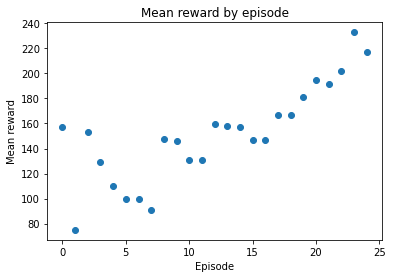
\includegraphics{img/SpaceInvaderRewards.png}
		\caption{Evolutionary Strategy's Rewards}
		\label{fig:SpaceInvaderRewards}
	\end{center}
\end{figure}

From Fig. \ref{fig:SpaceInvaderRewards} we see that generally the mean rewards increase as it goes through training (roughly nine hours worth on my PC, with no GPU usage). In the video (in videos/SpaceInvaders.mp4) we can see that the model scores 30 more points than one which we built in the notebook which simply executed a completely random action. Altogether that is not too suprising, as the model is built from multiple generations of neural networks based upon previous networks which had scored highly, rather than a deliberate policy of trying to improve the network. This critisism also applies somewhat to the Deep Q network models, as there currently is not a way to give the model an ovrview of what you want it to do (e.g. in Space Invaders destroy all of the ships and don't get killed) and let it start training from that (or to transfer the knowledge of playing similar games into this one). The other critisism is that with a human agent playing the game you could ask them why did you press that button and get at least an understandable response, with both Deep Q and Evolutionary Strategies the answer is that from running the array of values from the current state through the neural network produced an array of probabilities for several actions and then itselected the best one.
For a computer game such as this there is no regulatory need to provide the reasoning behind an action. If our model was buying or selling stocks on behalf of other people, driving a car/ship/plane, then regulators/auditors/accident investigations would want or legally require an explanation somewhat better than "the model said so".
In the video, we can see that the model is fairly good at the game (and may possibly be blessed with inhuman reflexes), but seems keen on shooting its own defenses and does not seem to have picked up the idea that you need to dodge the incoming laser blasts.

\section{Implementation of PPO or SAC}

\section{Summary of contribution}
100\% me

\bibliographystyle{agsm} % using https://www.imperial.ac.uk/media/imperial-college/administration-and-support-services/library/public/LaTeX-example-Harvard-apr-2019.pdf to get Harvard style references
\bibliography{MyLibrary}
\end{document}